\section{Evietania - 1174051}

\subsection{Teori}
\begin{enumerate}
\item Jelaskan apa itu random forest, sertakan gambar ilustrasi buatan sendiri.\par
Random Forest atau hutan acak yaitu kumpulan dari pohon-pohon keputusan yang digunakan untuk membaca objek tertentu yang telah di sepakati untuk di baca dalam AI. pohon-pohon keputusan tersebut akan memunculkan hasil-hasil yang akan disimpulkan oleh random forest. pembagian jumlah data yang dimasukan kedalam decision tree pada random forest akan di bagi sama rata sesuai codingan atau ketentuan tertentu yang di sepakati. misalkan data yang akan digunakan sebanyak 314 jika dalam satu decision tree di putuskan untuk memiliki 50 data maka pada satu random forest akan terdapat enam atau tujuh decision tree.
\begin{figure}[ht]
\centering
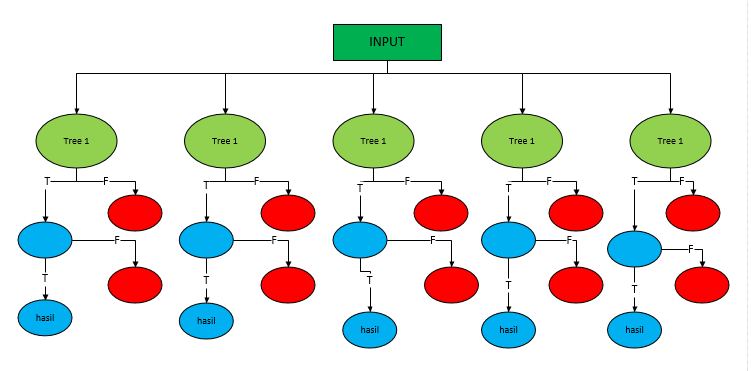
\includegraphics[scale=0.2]{figures/1174051/3/1.png}
\caption{contoh binari calssification}
\label{contoh}
\end{figure}

\item Jelaskan cara membaca dataset khusus dan artikan makna setiap file dan isi field masing masing file.
langkah pertama download terlebih dahulu dataset nya kemudian buka menggunakan spyder bawaan anaconda untuk mengetahui isi dari dataset tersebut. biasanya data tersebut berisi databerekstensi .txt yang di dalammya terdapat class dari field atau data data yang ada data tersebut. contoh pada data burung ada field index dan angka, index biasanya berisi angka, angka angka tersebut memiliki makna yaitu pengganti nama atau jenis dari burung tersebut sedangkan pada field yang berisi nilai 0 dan 1 berarti menyatakan atau maknanya yaitu memberikan nilai ya dan tidak nilai tersebut di ubah menjadi angka nol dan satu karna data pada field tersebut harus berisi nilai boolean atau pilihan ya dan tidak di karenakan komputer susah membaca nilai dan tidak maka di ubahlah menjadi 0 dan 1 dengan 0 bernilai tidak dan 1 bernilai ya.

\item Jelaskan apa itu Cross Validation.
Cross Validation merupakan cara untuk mengevaluasi hasil dari sebuah metode yang telah digunakan dengan cara membagi dua bagian dari dataset menjadi data training dan data testing kemudian data tersebut diolah hingga muncul tingkat akurasi dari metode yang digunakan contoh pada metode random forest dataset nya di bagi menjadi dua menjadi data training dan data testing kemudian data tersebut di olah oleh mesin untuk melihat tingkat akurasinya maka akan muncul misalkan akurasi kebenaran sebesar 44 \% begitu pula dengan menggunakan metode-metode yang lain seperti decision tree dan SVM.


\item Jelaskan apa arti score 44 \% pada random forest, 27 \% pada decision tree dan 29 \% dari SVM.
maksud dari score 44 \% tersebut yaitu nilai ketepatan atau kebenaran atau bisa disebut hasil dari random forest misalkan dengan metode random forest mesin membaca objek burung, mesin tersebut bisa menyatakan jenis burung tersebut dengan akurasi kebenaran 44 \%. sedangkan pada metode decision tree yaitu 27 \% yang berarti menunjukan bahwa tingkat akurasi ketepatan mesin jika mengerjakan sesuatu atau menyatakan keputusan dengan metode decision tree maka nilai kebenarannya bernilai 27 \%. sedangkan dengan menggunakan metode SVM menunjukan hasil 29 \% yang berarti nilai ketepatan atau kebenaran dalam memecahkan masalah menggunakan metode SVM ini sebesar 29 \% . maka dari itu dapat di simpulkan bahwa dengan menggunakan metode random forest mesin dapat memecahkan masalah lebih akurat dibandingkan dengan menggunakan decision tree dan SVM.


\item Jelaskan bagaimana cara membaca confusion matriks dan contohnya memakai gambar atau ilustrasi sendiri.
cara membaca confusioo matrix dengan cara memasukan para meter nilai yang ada pada datasets contoh pada dataset terdapat class yang disandingkan dengan nama burung untuk di normalisasi maka akan menunjukan nilai matrix yang mendekati nilai benar dalam bentuk angka misalkan 0,5 0,2 dan seterusnya mendekati nilai satu. di karenakan susahnya membaca nilai angka maka sering di ubah menjadi bentuk grafik. 
\begin{figure}[ht]
\centering
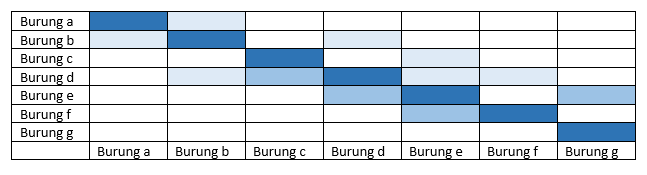
\includegraphics[scale=0.2]{figures/1174051/3/2.png}
\caption{contoh binari calssification}
\label{contoh}
\end{figure}

\item Jelaskan apa itu voting pada random forest disertai dengan ilustrasi gambar sendiri.\par
Voting merupakan data hasil dari decision tree yang terdapat pada random forest. Dimana hasil data tersebut di gunakan sebagai acuan untuk hasil dari random forest. sebagai contoh misalkan pada satu random forest terdapat enam decision tree untuk menentukan jenis pekerjaan orang, pada decision tree ke satu menyimpulkan bahwa pekerjaanya yaitu dosen , pada decision tree ke dua yaitu dosen kemudian pada decision tiga dosen , pada decision tree ke empat yaitu pekerja kantoran, pada decision tree ke lima yaitu pekerja kantoran dan pada decision tree ke enam yaitu dosen. maka pada random forest dapat menyimpulkan hasilnya yaitu dosen. 
\begin{figure}[ht]
\centering
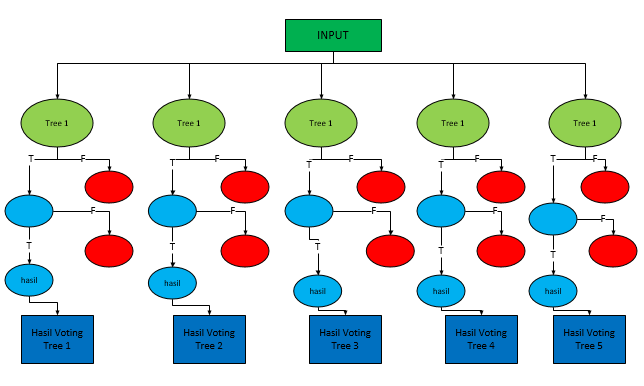
\includegraphics[scale=0.2]{figures/1174051/3/3.png}
\caption{contoh binari calssification}
\label{contoh}
\end{figure}

\end{enumerate}


\subsection{Praktikum}
\begin{enumerate}
\item pandas \par
pada baris ke satu yaitu perintah mengimport library padas pada python atau anaconda kemudian di inisialisasikan menjadi kue. selanjutnya pada baris ke 3 terdapat nama variabel yaitu nama\_kue\_tradisional = yang di dalammyanya terdapat tiga nama field yakni Name Kue, harga satuan dan terbilang kemudian pada baris ke tujuh terdapat variabel baru bernama Data\_kue = kemudian didalammnya mendeskripsikan kue berdasarkan tipe DataFrame yang berisi variabel nama\_kue\_tradisional selanjutnya data tersebut di cetak pada console dengan perintah print (Data\_kue).
\lstinputlisting{src/1174051/3/1.py}
\begin{figure}[ht]
\centering
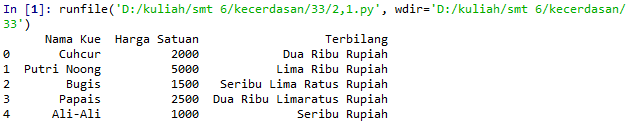
\includegraphics[scale=0.5]{figures/1174051/3/4.PNG}
\caption{hasil}
\label{contoh}
\end{figure}

\item numpy\par
Arti tiap baris codingan pada aplikasi sederhana numpy adalah sebagai berikut : pada baris ke satu yaitu mengimport numpy yang di inisialisasi menjadi np kemudian pada baris ke tiga dibut variabel ali yang berisi numpy bertipekan arrange 6 yang berarti berisi nilai array dari 0 sampai 5 kemudian pada baris ke empat di cetak hasilnya dengan memasukan perintah print (ali) selanjutnya yaitu membuat nilai array tiga dimensi pada baris ke tujuh dengan cara membuat variabel botak yang berisi rank nilainya kemudian dimensinya yaitu 4 3 3 kemudian variabel tersebut di print. selanjutnya pada baris ke 12 dibuat variabel nilai\_array\_1 dengan isian nilai array 1 2 3 4 kemudian pada baris ke 13 di buat variabe nilai\_array\_2 dengan nilai array 20 30 40 dan 50 selanjutnya pada baris ke 14 dibut nilai variabel Nilai\_array\_3 dengan rank 4 yang berarti berisi nilai dari 0 sampai 3 setelah itu di buat variabel hasil dimana isinya yaitu penjumlahan nilai\_array\_1+Nilai\_array\_3+Nilai\_array\_3 setelah itu nilai\_array\_1 , Nilai\_array\_3, dan Hasil di prin untuk melihat nilai dari array tersebut.
\lstinputlisting{src/1174051/3/2.py}
\begin{figure}[ht]
\centering
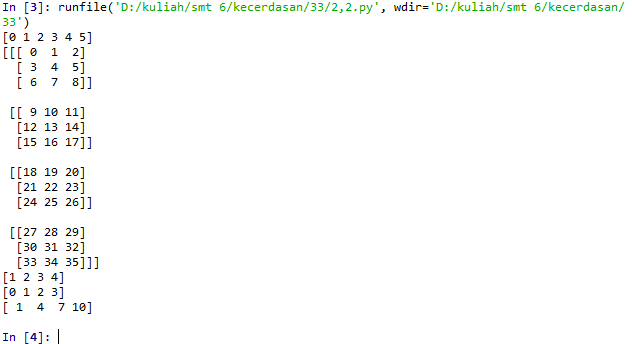
\includegraphics[scale=0.5]{figures/1174051/3/5.PNG}
\caption{hasil}
\label{contoh}
\end{figure}

\item matplotlib\par
Arti tiap baris aplikasi sederhana matplotlib pada baris ke satu yaitu memasukan library matplotlib.pyplot yang di definisikan menjadi plt kemudian membuat variabel kelas\_ti3 pada baris ke tiga yang berisi label setelah itu di buat variabel jumlah\_mhs3 pada baris ke empat yang berisi nilai dari setiap label tersebut. begitu juga pada baris ke emam dan ke tujuh kemudian pada baris ke sembilan matplotlib mendefinisikan gambar dengan ukurannya dan pada baris ke 10 di dekralasikan subplot setelah itu pada baris ke 11 matplotlib mendefinisikan jenis grafik yang digunakan dan dimasukan variabel kelas dan jumlah\_mhs. begitujuga oada baris ke 13 14 dan 15 setelah itu di buat title  pada baris ke 17 dan matplotlib di show untuk mendapatkan hasil dari grafiknya.
\lstinputlisting{src/1174051/3/3.py}
\begin{figure}[ht]
\centering
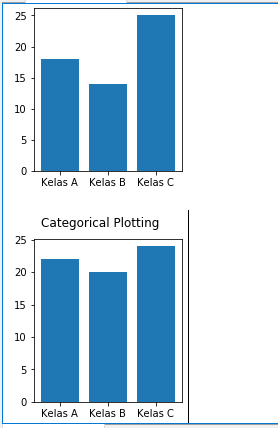
\includegraphics[scale=0.5]{figures/1174051/3/6.PNG}
\caption{hasil}
\label{contoh}
\end{figure}

\item Random Forest\par
Arti tiap baris hasil codingan random forest pada baris pertama random forest di import dari sklearn dengan ketentuan yaitu maksimal isi dari decision tree berisi 50 data dengan keadaan random dan dengan estimators 100 data ini berada dalam variabel clf kemudian setelah itu variabel clf di running berdasarkan data training dan data label yang telah di definisikan jumlahnya. kemudian variabel clf di running berdasarkan data training paling atas untuk memunculkan hasil data training lima paling atas. setelah itu data tersebut di di running scorenya untuk melihat tingkat akurasi yang dia kerjakan maka tingkat akurasi yang dihasilkan berada pada kisaran 0,437 atau kisaran 43 \%.
\lstinputlisting{src/1174051/3/4.py}
\begin{figure}[ht]
\centering
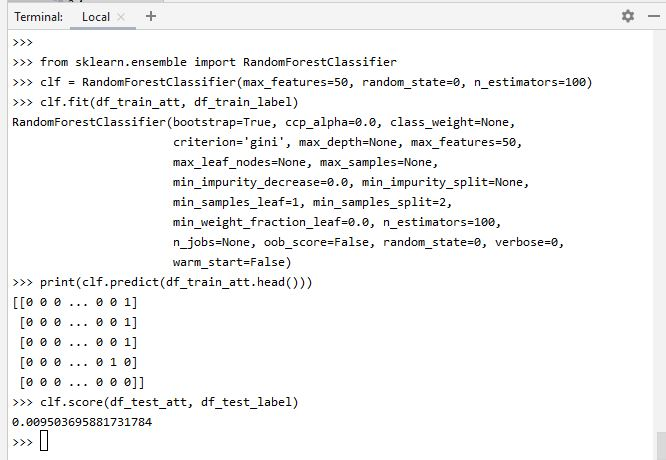
\includegraphics[scale=0.5]{figures/1174051/3/7.JPG}
\caption{hasil}
\label{contoh}
\end{figure}

\item Confusion Matrix\par
arti codingan pada hasil tiap codingan confusion matrix pada baris pertama codingan tersebut mendeskripsikan atau mengimport confusion matrix dari sklearn kemudian dibuat variabel pred labels dengan di isikan clf prdic df\_test\_att setelah itu membuat variabel cm yang isinya terdapat data yang di buat confusion matrix berdasarkan data test setelah variabel cm akan di running yang mana akan menghasilkan gambar berupa matrix matrix tersebut berisi nilai nilai kebenaran yang mendekati nilai benar atau mutlak nilai benar.
\lstinputlisting{src/1174051/3/5.py}
\begin{figure}[ht]
\centering
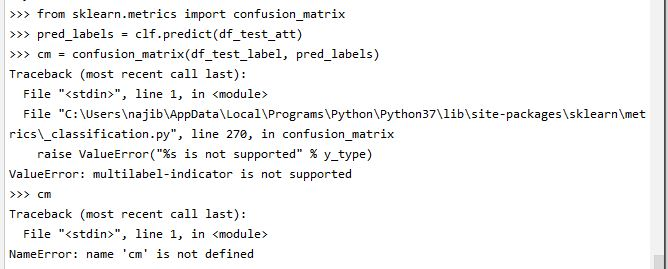
\includegraphics[scale=0.5]{figures/1174051/3/8.JPG}
\caption{hasil}
\label{contoh}
\end{figure}

\item SVM dan Decision Tree\par
Arti dari setiap baris hasil codingan decision tree dan SVM pada tree masukan terlebih dahulu library tree setelah itu buat variabel clftree yang berisi decision tree setelah itu masukan nilai data training dan label yang telah di deklarasikan tadi setelah itu running variabel tersebut untuk mendapatkan score 0,266 kisaran 26 sampai 27 \% akurasinya kemudian pada svm juga hampirsama masukan terlebih dahulu librarynya setelah itu buat variabel clfsvm yang berarti berisi nilai data training dan data label dan pendeklarasian svm itu sendiri setelah itu di running untuk mendapatkan nilai akurasinya atau score sebesar 0,283 atau dalam kisaran 23 \%.
\lstinputlisting{src/1174051/3/6.py}
\begin{figure}[ht]
\centering
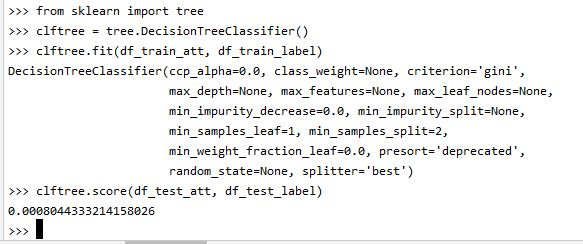
\includegraphics[scale=0.5]{figures/1174051/3/9.JPG}
\caption{hasil}
\label{contoh}
\end{figure}

\item Cross Validation\par
arti dari setiap baris hasil cross falidation pada gambar\ref{c47} tersebut diperlihatkan codingan error dikarenakan data training terlalu besar maka untuk mengatasi halini dapat dlilihat pada sub bab penanganan error 
\lstinputlisting{src/1174051/3/7.py}
\begin{figure}[ht]
\centering
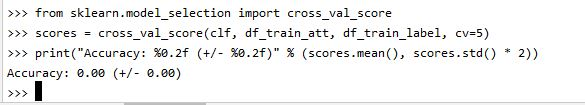
\includegraphics[scale=0.5]{figures/1174051/3/10.JPG}
\caption{hasil}
\label{contoh}
\end{figure}

\item program pengamatan
arti dari hasil program pengamatan. perogram pengamatan ini menggunakan library matplotlib supaya hasil dari presentase hasil random forest, svm dan decision tree dapat di bandingkan dengan membuat variabel X Y Z kemudian memberikan label untuk setiap dimensinya untuk lebih jelas dapat dilihat gambar \ref{c48} yang menunjukan hasil perbandingan presentase dari tiga metode tersebut. 
\lstinputlisting{src/1174051/3/8.py}
\begin{figure}[ht]
\centering
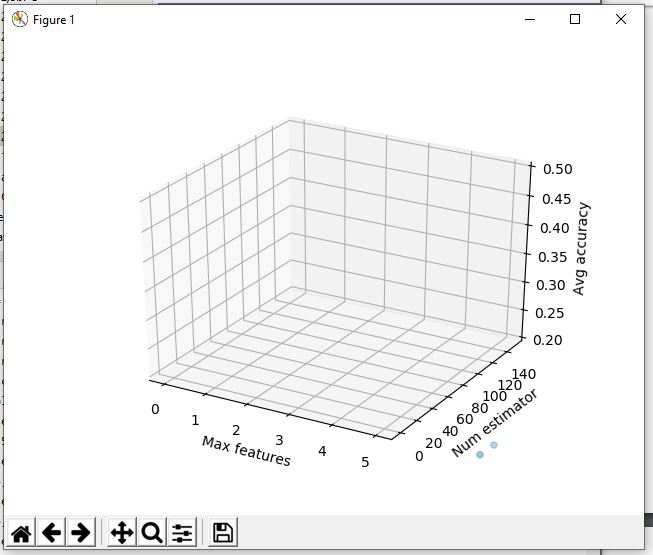
\includegraphics[scale=0.5]{figures/1174051/3/11.JPG}
\caption{hasil}
\label{contoh}
\end{figure}
\end{enumerate}


\subsection{Penanganan Error}
Screenshot error
\begin{enumerate}
\item  Untuk gambar screenshot error
\begin{figure}[ht]
\centering
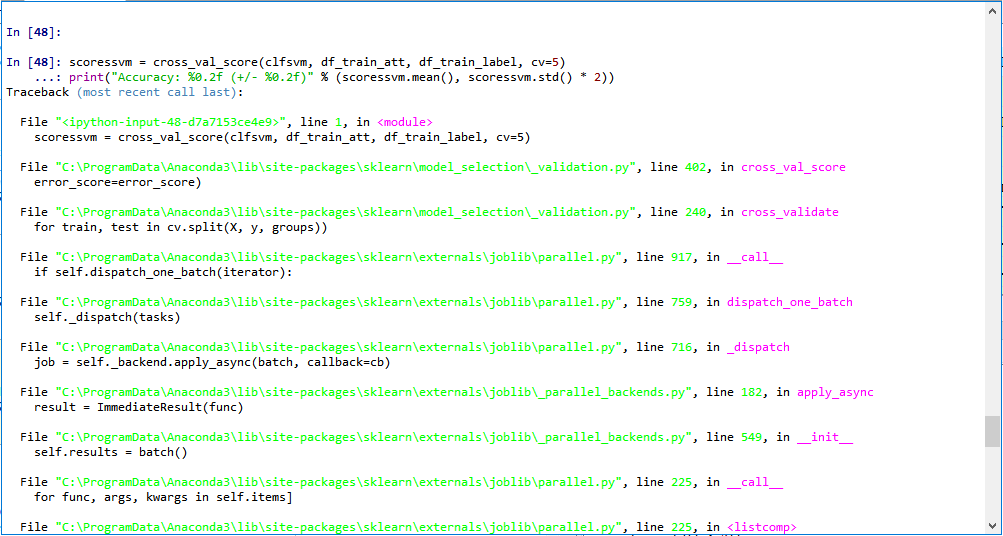
\includegraphics[scale=0.5]{figures/1174051/3/error/error.PNG}
\caption{hasil}
\label{contoh}
\end{figure}
\end{enumerate}

Code Errornya 
\begin{enumerate}
\item kode error pada screenshot ke satu yaitu dikarenakan clfsvm.fit(df\_train\_att, df\_train\_label) dikarenakan data trainingnya terlalu besar sehingga komputernya error.
\item untuk kode error pada screen shoot ke 2 sampai ke 4 dikarenakan pada kode berikut  scores = cross\_val\_score(clf, df\_train\_att, df\_train\_label, cv=5) scorestree = cross\_val\_score(clftree, df\_train\_att, df\_train\_label, cv=5) dan  
scoressvm = cross\_val\_score(clfsvm, df\_train\_att, df\_train\_label, cv=5) hal ini di karenakan data trainingterlalu besar sehingga berdampak pada komputer sehingga library dari python tidak mampu mengolah data dan hasilnya menjadi error. 
\end{enumerate}

Solusi Untuk mengatasi Error
\begin{enumerate}
\item solusinya untuk yang ke satu yaitu dengan cara merestart spyder atau mematikannya kemudian nyalakan kembali lalu jalankan code yang error tersebut di CMD cika dalam python CMD jalam maka bisa di running. setelah itu buka kembali spyder dan jalankan codingan dari awal hingga pada bagian SVM tunggu sebenar sampai muncul nilai akurasinya.
\item solusi untuk mengatasi error tersebut yaitu dengan cara merubah bobot data pada data training.
\begin{figure}[ht]
\centering
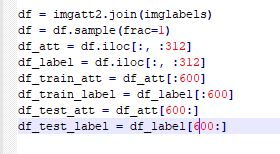
\includegraphics[scale=0.5]{figures/1174051/3/plagiat/plagiat.JPG}
\caption{hasil}
\label{contoh}
\end{figure}
\end{enumerate}